

Let $Y_1$ and $Y_2$ be two independent and identically distributed (IID) uniform random variables.\\
Let X be a random variable such that
\begin{align}
    X = Y_1 + Y_2
\end{align}
Let
\begin{align}
    p_{Y_1}\brak{y} &= \Pr\brak{Y_1=y} \\
    p_{Y_2}\brak{y} &= \Pr\brak{Y_2=y} \\
    p_X\brak{x} &= \Pr\brak{X=x}
\end{align}
be the probability densities of random variables $Y_1, Y_2$ and $X$. \\
$Y_1$ and $Y_2$ lie in the range \brak{\frac{-c}{4},\frac{c}{4}}, therefore, the PDF for $Y_1$ and $Y_2$,
\begin{align}
p_{Y_1}\brak{y} = p_{Y_2}\brak{y} = 
\begin{cases}
\frac{2}{c} &  \frac{-c}{4} \le y \le \frac{c}{4}\\
0 & \text{otherwise}
\end{cases}
\end{align}

The density of X is obtained by convolution of $Y_1$ and $Y_2$
\begin{align}
p_X\brak{x} = p_{Y_1}(x)*p_{Y_2}(x)
\end{align}
where $*$ denotes the convolution operation. Since convolution operation is time invariant, 
\begin{multline}
    p_X\brak{x-t} = p_{Y_1}(x-t)*p_{Y_2}(x) \\ = p_{Y_1}(x)*p_{Y_2}(x-t)
\end{multline}
On time shifting $Y_1$ by shifting factor $t=a+\frac{c}{2}$, 
\begin{align}
    p_X\brak{x-\brak{a+\frac{c}{2}}} =  p_{Y_1}\brak{x-\brak{a+\frac{c}{2}}}*p_{Y_2}\brak{x}
\end{align}
Thus, the PDF of time shifted X obtained by convolution is,
\begin{align}
p_x = 
\begin{cases}
\frac{4}{c^2}\brak{x-a} & a \le x \le a+\frac{c}{2}\\
\frac{4}{c^2}\brak{a+c-x} & a+\frac{c}{2} \le x \le a+c \\
0 & \text{otherwise}
\end{cases}
\end{align}

On comparing the parameters of PDF of time shifted X with that in the question, we have

\begin{align}
    b=\frac{c}{2}\\
    a=\frac{2}{c}
\end{align}
\rightline{Answer : Option A}


\begin{figure}[!ht]
\centering
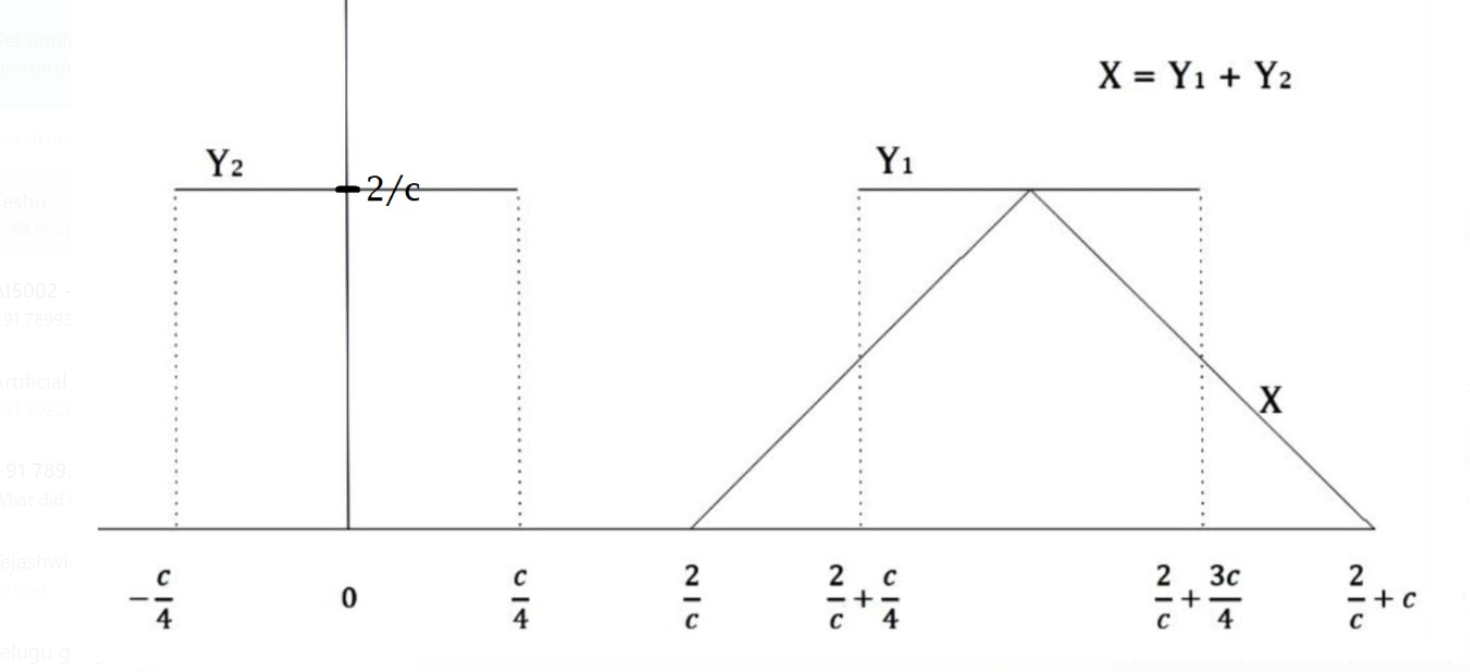
\includegraphics[width=\columnwidth]{solutions/in/2006/2/figures/con6.png}
\caption{PDF of time shifted X}
\label{in2006-2:fig:convolution}
\end{figure}
The following are some observations: 
\begin{enumerate}
    \item The sum of two equally distributed random variables will lead to a triangular probability density
    \item The two uniformly distributed random variables lie in the range $\brak{\frac{-c}{4},\frac{c}{4}}$ and $\brak{\frac{2}{c}+\frac{c}{4} , \frac{2}{c}+\frac{3c}{4}}$. \\
    \because $X = Y_1 + Y_2$ the range of X is thus $\brak{\frac{2}{c},\frac{2}{c}+c}$
    \item On time shifting $Y_1$ to the right by a factor $a+\frac{c}{2}$, the convoluted PDF of X also shifts by the same factor without any change in it's width.
\end{enumerate}

Fig \ref{in2006-2:fig:sim1} and Fig \ref{in2006-2:fig:sim2} are the simulated plots of PDF and CDF obtained by taking c=2
\begin{figure}[h!]
\centering
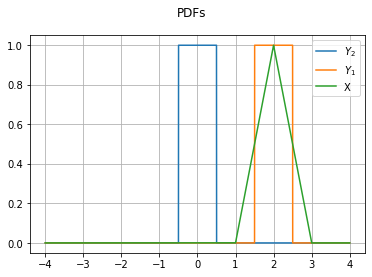
\includegraphics[width=\columnwidth]{solutions/in/2006/2/figures/sim1.png}
\caption{PDF of $Y_1, Y_2$ and X}
\label{in2006-2:fig:sim1}
\end{figure}
\begin{figure}[!ht]
\centering
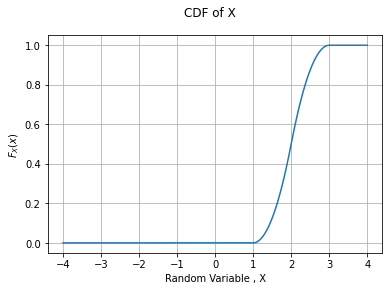
\includegraphics[width=\columnwidth]{solutions/in/2006/2/figures/sim2.png}
\caption{CDF of X}
\label{in2006-2:fig:sim2}
\end{figure}


\end{document}
